%
% File acl2017.tex
%
%% Based on the style files for ACL-2015, with some improvements
%%  taken from the NAACL-2016 style
%% Based on the style files for ACL-2014, which were, in turn,
%% based on ACL-2013, ACL-2012, ACL-2011, ACL-2010, ACL-IJCNLP-2009,
%% EACL-2009, IJCNLP-2008...
%% Based on the style files for EACL 2006 by 
%%e.agirre@ehu.es or Sergi.Balari@uab.es
%% and that of ACL 08 by Joakim Nivre and Noah Smith

\documentclass[11pt,a4paper]{article}
\usepackage[hyperref]{acl2017}
\usepackage{times}
\usepackage{latexsym}
\usepackage{xcolor}
\usepackage[normalem]{ulem}
\usepackage{url}
\usepackage{caption}
\usepackage{subcaption}
\usepackage{pgfplots}
\usepackage{tikz}

\definecolor{forestgreen}{rgb}{0.13, 0.55, 0.13}

% Define bar chart colors
%
\definecolor{bblue}{HTML}{4F81BD}
\definecolor{rred}{HTML}{C0504D}
\definecolor{ggreen}{HTML}{9BBB59}
\definecolor{ppurple}{HTML}{9F4C7C}

%\aclfinalcopy % Uncomment this line for the final submission
%\def\aclpaperid{***} %  Enter the acl Paper ID here

%\setlength\titlebox{5cm}
% You can expand the titlebox if you need extra space
% to show all the authors. Please do not make the titlebox
% smaller than 5cm (the original size); we will check this
% in the camera-ready version and ask you to change it back.

\newcommand\BibTeX{B{\sc ib}\TeX}

% Writing macros
\newcommand{\secref}[1]{Section~\ref{ssec:#1}}
\newcommand{\figref}[1]{Figure~\ref{#1}}
\newcommand{\tabref}[1]{Table~\ref{#1}}
\newcommand{\isection}[2]{\section{#1}\label{ssec:#2}}
\newcommand{\isectionb}[1]{\section{#1}\label{ssec:#1}}
\newcommand{\com}[1]{}
\newcommand{\resolved}[1]{}
% Editing macros
\newcommand{\my}[1]{\footnote{\color{red}{\textbf{#1}}}}

\newcommand{\ms}[1]{{\color{cyan}\{\textit{#1}\}$_{ms}$}}
\newcommand{\roy}[1]{{\color{orange}\textsc{[#1 --rs]}}}
\newcommand{\royb}[2]{{\color{red}{\sout{#1}}}{\color{green}{#2}}}
\newcommand{\royc}[3]{\royb{#1}{#2}\roy{#3}}
\newcommand{\yc}[1]{{\color{bblue}\{\textit{#1}\}$_{yc}$}}
\newcommand{\nascomment}[1]{{\color{blue}\textsc{[#1 --nas]}}}
\newcommand{\clinic}[1]{{\color{magenta}\textsc{[#1 --CLINIC]}}}

%\renewcommand{\ms}[1]{}
%\renewcommand{\roy}[1]{}
%\renewcommand{\nascomment}[1]{}
%\renewcommand{\yc}[1]{}
%\renewcommand{\royb}[1]{}
%\renewcommand{\royc}[1]{}


\title{The Effect of Different Writing Tasks on Linguistic Style:\\ A Case Study of the ROC Story Cloze Task}

\author{First Author \\
  Affiliation / Address line 1 \\
  Affiliation / Address line 2 \\
  Affiliation / Address line 3 \\
  {\tt email@domain} \\\And
  Second Author \\
  Affiliation / Address line 1 \\
  Affiliation / Address line 2 \\
  Affiliation / Address line 3 \\
  {\tt email@domain} \\
  }

\date{}

\begin{document}
\maketitle
\begin{abstract}
%People's writing style is affected by many factors, including topics, sentiment, and individual personality. 
% People's writing style depends not just on the authors' personal
% traits but also on the intent and the cognitive states of the
% authors. 
A writer's style depends not just on personal traits but also on her intent and mental state.
%In this paper we show that engaging authors in different  writing tasks results in them adopting different writing styles.
In this paper, we show how variants of the same writing task can lead to measurable differences in writing style. % of the same authors.  
We present a case study based on 
the  {\it story cloze task} \cite{Mostafazadeh:2016},
where annotators were assigned similar writing tasks with different constraints: (1) writing an entire story, (2) adding a story ending for a given story context, and (3) adding an incoherent ending to a story.\resolved{\clinic{Many felt these 2 constraints looks like 3 constraints. clarify}}
%We show that a linear classifier, which applies only simple style features, such as sentence length and character n-grams, 
We show that a simple linear classifier informed with stylistic features is able to successfully distinguish between the three cases, without even looking at the story context.
In addition, our style-based classifier establishes a new state-of-the-art result on the story cloze challenge, substantially higher than previous results based on deep learning models. 
%Furthermore, combining our model with an LSTM-based language model, which does look at the context, leads to additional gains.
Our results demonstrate that different task framings can dramatically affect the way people write.\resolved{\clinic{Similarly to previous comment: which results does this comment address?}}


\resolved{They also provide important lessons for designing new NLP
tasks. \nascomment{drop this sentence if we only have a paragraph
  about this at the end, as we currently do}}

\end{abstract}

\section{Introduction}
Writing style is expressed through a range of linguistic elements such as words, sentence structure, and rhetorical devices.
It is influenced by both personal factors such as age \cite{Schler:2006} and gender \cite{Argamon:2003}, 
by personality traits such as agreeableness and openness  \cite{Ireland:2014b},
as well as by mental states\resolved{\clinic{Avoid using ``cognitive"?}} such as sentiment \cite{Davidov:2010}, sarcasm \cite{Tsur:2010}, and deception \cite{Feng:2012}.  
In this paper, we study the extent to which writing style is affected by the nature of the writing task the writer was asked to perform, since
different tasks likely engage different cognitive processes \cite{Campbell:2003,Banerjee:2014}.

\begin{table}[!t]
%\small
\begin{tabular}{|p{1.6cm}|p{5.3cm}|} \hline
{\bf Type} & {\bf Example} \\ \hline
{\color{blue}{Original}} story & My mother loves clocks that chime.	Her house is full of them.	She sets them each a little different so she can hear them chime.	It sounds like a bell tower during a wedding in her house all day.	{\color{blue}{When I visit I stop them or I'd never be able to sleep at night.}} \\ \hline
{\color{forestgreen}{Coherent}} story & Kathy went shopping.	She found a pair of great shoes.	The shoes were \$300.	She bought the shoes.	{\color{forestgreen}{She felt buyer's remorse after the purchase.}} \\ \hline
{\color{red}{Incoherent}} story & Kathy went shopping.	She found a pair of great shoes.	The shoes were \$300.	She bought the shoes.	{\color{red}{Kathy hated buying shoes.}} \\ \hline
\end{tabular}
\caption{\label{ROC-example}
Examples of stories from the story cloze task \cite{Mostafazadeh:2016}. The first row shows an {\color{blue}{original}} story written by one author. 
The second and third rows show revised stories with two contrastive endings:
 %of the same story: 
 a {\color{forestgreen}{coherent}} ending and a {\color{red}{incoherent}} one.\resolved{ \clinic{They said it would be great to have three endings to the same story. Unfortunately Nasrin et al.  didn't publish the original endings for the dev/test data. We could ask her, but not sure if this is worth it}}
 \resolved{\nascomment{I like the colors a lot.  Instead of all the italicizing,
let's consider just color-coding these three terms.  It's less distracting.}}
}
%\end{center}
\end{table}

We show that similar writing tasks with different constraints on the author can lead to measurable differences in people's writing style.
%We explore three  writing tasks, showing that they are distinguishable from one another using a linear classifier informed with stylistic features only. 
%Our results hint that different writing tasks impose different cognitive load on the writer, which lead to the substantial style differences.
As a case study, we present experiments   based on 
the recently introduced ROC story cloze task \cite{Mostafazadeh:2016}. 
In this task, \com{crowdsourced }authors were asked to write five-sentence self-contained stories, henceforth {\it original} stories.
%Following, 
Then, 
%the stories were given to other authors, 
each original story was given to a different author, 
who was shown only the first four sentences as a story context, 
and asked to write contrastive story endings: a {\it right} (coherent) ending, and a {\it wrong} (incoherent) ending. 
Framed as a story cloze task, the goal of this dataset is to serve as a commonsense challenge for NLP and AI research. 
\tabref{ROC-example} shows an example of an {original} story, a {coherent} story, and an {incoherent} story.

\com{While originally designed to be a story understanding challenge, the annotation process triggers interesting questions 
that may go beyond the original intent of the designers.
First, do people maintain the same writing 
style when asked to write both coherent and incoherent story endings? 
Second, do people maintain the same writing style when writing the entire story on their own compared to 
writing only the final sentence for a given story context written by someone else? }

\com{
%Our analysis indicates that the answer to both questions is positive. 
Our analysis indicates that different framings of similar writing tasks 
can lead to measurable differences in people's writing style.\clinic{This is the main message -- should come earlier}
%We experiment with a linear classifier, using simple stylistic features, such as sentence length, character n-grams and word n-grams. 
%First, we show that on a balanced dataset (chance level is 50\%) our classifier distinguishes between the {\it right} and {\it wrong} endings in 64.5\% of the cases. 
Using a simple classifier informed with stylistic features, we show that our classifier can distinguish the {\it right} and {\it wrong} endings with 64.5\% accuracy, even without looking at the story context, where chance performance is 50\%.
%It is also trained on a set of positive samples and a set of negative ones, rather than pairs of (positive, negative) pairs, as in the original story cloze task.
%Second, when trained to distinguish between the {\it original} endings and the new ({\it right}) endings, the classifier obtains 68.5\% accuracy. 
Further, our classifier can also distinguish between the {\it original} endings and the new ({\it right}) endings with 68.5\% accuracy, again without looking at the story context. \clinic{Why do we care? (Luke)}
}

\com{We show that a linear classifier informed with stylistic features can distinguish between {\it original}, {\it right} and {\it wrong}  endings to a large degree, even without looking at the story context.
Our results allow us to make a few key observations.
First, people adopt a different writing style when asked to write coherent vs.~incoherent story endings.
Second,  people change their writing style when writing the entire story on their own compared to 
writing only the final sentence for a given story context written by someone else.}

%Our binary classification results range between 64.5\%--75.6\%, where chance performance is 50\%.

%Importantly, in both experiments, the classifier uses {\bf only} the 
%last sentence of each of the stories, and does not consider the first four sentences.
%final sentence without the story context. 

While the story cloze task was originally designed to be a story understanding challenge, 
its annotation process introduced three variants of the same writing task: writing an {\it original}, {\it right} or {\it wrong} ending to a short story.
In this paper, we show that a linear classifier informed with stylistic features can distinguish between the different endings to a large degree, even without looking at the story context (64.5\%--75.6\% binary classification results).

Our results allow us to make a few key observations.
First, people adopt a different writing style when asked to write coherent vs.~incoherent story endings.
Second,  people change their writing style when writing the entire story on their own compared to 
writing only the final sentence for a given story context written by someone else.


In order to further estimate the quality of our results, we also directly tackle the story cloze challenge. 
 Adapting our classifier to the task, we obtain 72.4\% accuracy, a 12.5\% increase over the previously reported state-of-the-art  \cite{Salle:2016}.
We also show that the style differences captured by our model can be combined with neural language models to make a better use of the story context. 
Our final model that combines context with stylistic features achieves
75.2\%---an additional 2.8\% gain, 15.3\% better than the best
published result.

\com{Our results suggest that writing style is affected by the the writer's state of mind.
Writing a sentence intended to be {\it wrong} turns out quite differently than a sentence intended to be {\it right}. 
Similarly, writing a sentence as part of the story is different from reading a story, and then writing the final sentence.}

The contributions of our study are threefold. 
First, findings from our study can potentially shed light on 
how different kinds of cognitive load influence the style of written language. 
Second, our results indicate that when designing new NLP tasks, special attention needs to be payed to the instructions given to authors.
%both in terms of the potential impact of even the smallest details, and the need to carefully run baseline models.
Third, we establish a new state-of-the-art result on the commonsense story cloze challenge. 

\com{
The remainder of this paper is organized as follows. In \secref{ROC_Story} we describe the story cloze task.
We then present our model, experiments and results in Sections \ref{ssec:Model}, \ref{ssec:Experiments} and \ref{ssec:Results} respectively.
Sections \ref{ssec:Ablation} and \ref{ssec:Discussion} present a further analysis of our results  and a discussion, followed by related work and conclusions.\clinic{Omit this paragraph?}}

\isection{Background: The Story Cloze Task}{ROC_Story}
To understand how different writing tasks affect writing style, 
we focus on the \textit{story cloze task} \cite{Mostafazadeh:2016}. 
While this task was developed to facilitate representation and learning of commonsense story understanding,
its design included a few key choices which  make it ideal for our study. 
We describe the task below.


%For that purpose, \citet{Mostafazadeh:2016} crowdsourced the collection of two types of datasets: the \textit{ROC Stories} and the \textit{Story Cloze test sets}.


\paragraph{ROC stories.}

The ROC story corpus consists of 49,255 five-sentence commonsense stories, collected on Amazon Mechanical Turk (AMT).\footnote{Recently, an additional 53K stories were released, which results in roughly 100K stories.}
Workers were instructed to write a coherent self-contained story, which has a clear beginning and end. 
To collect a broad spectrum of commonsense knowledge, there was no imposed subject for the stories,
which resulted in a wide range of different topics.

\paragraph{Story cloze task.}
After compiling the story corpus, the {\it story cloze task}---a task based on the corpus---was introduced.
A subset of the stories was selected, and only the first four sentences of each story were presented to AMT workers.
Workers were asked to write a pair of new story endings for each story context: one {\it right} and one {\it wrong}.
Both endings are required to complete the story using one of the characters in the story context. 
Additionally,  the ending is required to be ``realistic and sensible'' \cite{Mostafazadeh:2016} when read out of context.

The resulting stories, both {\it right} and {\it wrong}, were then individually rated for coherence and meaningfulness by additional AMT workers. \resolved{\nascomment{by
-  additional AMT workers? or someone else?}} 
Only stories rated as simultaneously coherent with a {\it right} ending and neutral with a {\it wrong} ending were selected for the task. 
It is worth noting that workers rated the stories as a whole, not only the endings.

Based on the new stories, \citet{Mostafazadeh:2016} proposed the {\it story cloze task}. 
The task is simple:  given a pair of stories that differ only in their endings, the system decides which ending is {\it right} and which is {\it wrong}. 
%The authors published the ROC story corpus as the training data, and the task composed of development and test sets for which both {\it right} and {\it wrong} endings are found. 
The official training data contains only the original stories (without alternative endings), while development and test data consist of the revised stories with alternative endings (for a different set of original stories that are not included in the training set).\roy{added {\it not} here} 
The task was suggested as an extensive evaluation framework:
%as a machine reading task, 
as a commonsense story understanding task, 
as the shared task for the  Linking Models of Lexical, Sentential and Discourse-level Semantics workshop (LSDSem 2017), and as a testbed for vector-space evaluation \cite{mostafazadeh2016story}.

Interestingly, at the time of this submission, 10 months after the
task was first introduced, the published benchmark on this task is
still below 60\% \cite{Salle:2016}.\footnote{The LSDSem 2017 shared
  task website (\url{https://competitions.codalab.org/competitions/15333}) does report higher results (71.1\%)\roy{Tricky. Which number should we report here? leave empty?}, which are still unpublished along with the underlying methodology.}
This comes in contrast to other recent similar machine reading tasks such as CNN/DailyMail \cite{hermann2015teaching}, SNLI \cite{bowman2015large}, LAMBADA \cite{Paperno:2016} and SQuAD \cite{rajpurkar2016squad}, for which results improved dramatically over a similar or shorter period of time.
This suggests that this task is challenging and that high performance is hard to achieve.
 \resolved{\yc{SQuAD was officially published in Nov 2016. by the time the official EMNLP talk was presented, the leaderboard performance (still unpublished) was  30\% beyond the best results in the paper. Given that, the statement of this paragraph seems a bit of overkill...?} \nascomment{it sounds like Yejin is saying that on squad, there was an even faster acceleration?  or that we should change ``similar period of time'' to ``similar or shorter period of time''?}}

In addition, \citet{Mostafazadeh:2016} made substantial efforts to ensure the quality of this dataset. 
First, each pair of endings was written by the same author, which ensured that author style differences could not be used to solve the task. 
Furthermore, the authors implemented nine baselines for the task, using surface level features as well as narrative-informed ones, and showed that each of them reached roughly chance-level.
These results indicate that real understanding of text is required in order to solve the task.

\paragraph{Different writing tasks in the story cloze Task.}
Several key design decisions make this task an interesting testbed for the purpose of this paper.\resolved{\clinic{Which purpose?}}
First, the training set for the task (ROC Stories corpus) is not a
training sample in the usual sense,\footnote{I.e., the training
  instances are not drawn from a population similar to the one that future
  testing instances will be drawn from.\roy{I added \textbf{not} here, as otherwise it is confusing}}  as it contains only positive ({\it right}) samples, and not negative ({\it wrong}) ones. 
 \resolved{\yc{As far as I understand, this was intentional --- they didn't want
  people to pick up on random superfluous cues that can inevidently
  get into the data creation process, exactly the kind that our work
  picks up. Given that, stating this can be viewed as
  misunderstanding, I'm afraid.} \nascomment{We should maybe say that
  they did this intentionally and concede that our approach goes
  against the intentions of their task design.  But a task that
  insists that systems avoid using features that might encode one kind
of information (like style) is absurd.  Alternately, we could reframe
this not as ``things weren't controlled for'' but instead stick to the
facts here and just describe what they did without judgment.}}

On top of that, the {\it original} endings, which serve as positive training samples, were generated differently from the {\it right} samples, which serve as the positive samples in the development and test sets. 
While the former are part of a single coherent story written by the same author, the latter were generated by letting an author read four sentences, 
and then asking her to generate a fifth {\it right} ending. 
%This raises the question of whether these different writing setups impose different writing styles. 
% We show that this is indeed the case. 

Finally, although the {\it right} and {\it wrong} sentences were generated by the same author, 
the tasks for generating them were quite different: in one case, the author was asked to write a {\it right} ending, which would create a coherent five-sentence story along with the other four sentences. In the other case, the author was asked to write a {\it wrong} ending, which would result in an incoherent five-sentence story. 
 \resolved{In this work, we show that these differences are significant and
impose different writing styles on authors. \nascomment{this bit feels
  a little heavy and reptititive.}}

\isection{Surface Analysis of the Story Cloze Task}{Surface}
We computed several characteristics of the three types of endings: {\it original} endings (from the ROC story corpus training set), {\it right} endings and {\it wrong} endings (both from the story cloze task development set).
Our analysis  reveals several style differences between different groups. 
First, {\it original} endings are on average longer (11 words per
sentence) than {\it right} endings (8.75 words), which are in turn
slightly longer than {\it wrong} ones (8.47 words). 
Previous work have shown that sentence length is also indicative of whether a text was deceptive \cite{yancheva2013automatic,qin2004exploratory}. 
Although writing {\it wrong} sentences is not the same as lying, it is not entirely surprising to observe similar trends in both tasks.
%Furthermore, \citet{Buller:1996} suggests lying increases one's cognitive load, which in turn could affect sentence length.
%\yc{Is there psycholinguistic literature that we can cite that may have shown that cognitive burden causes writers to write shorter sentences...?}

Second, \figref{roc_pos_distribution} shows the distribution of five frequent POS tags in all three groups. 
The figure shows that both {\it original} and {\it right} endings use pronouns more frequently than {\it wrong} endings.
Once again, deceptive text is also characterized by fewer pronouns compared to truthful text \cite{Newman:2003}.
%In contrast, {\it wrong} and {\it right} endings favor proper nouns compared to {\it original} endings. 
 \resolved{\yc{Is there literature that may have shown that (1) pronouns correlate with coherent text, and/or (2) referencing characters by proper nouns shows a way of cognitive distancing...?}}
 \resolved{\ms{The proper noun thing is prolly related to the task design, which stated that people had to use at least one of the characters; research shows people usually use more other references when lying, but it's not clear whether there's a pronoun/proper noun distinction.}}
  \resolved{\roy{Good point! This is tricky. On the one hand, it hurts our story by saying that the difference is not really the general task by itself, but also the constraints put by  Nasrin et al. It also forces us to bash them some more. Or we can just ignore it...} }
  \resolved{\yc{Ok! I resolved all comments above and also commented out the comment on how wrong/right endings use more proper nouns compared to the original endings. I think it's the best not to talk about this.}}

Finally, \figref{roc_word_distribution} presents the distribution of five frequent words across the different groups. 
The figure shows that {\it original} endings use coordinations (``and'') more than  {\it right} endings, and substantially more than {\it wrong} ones. %\ms{\cite{Newman:2003} found that liars use less ``contrast'' coordination, did we find that in our experiments?}.
Furthermore, {\it original} and {\it right} endings seem to prefer enthusiastic language (e.g., ``!''), while {\it wrong} endings tend to use more negative language (``hates''), similarly as deceptive text \cite{Newman:2003}.
%\yc{Again, any cogsci literature on this?} \nascomment{feels
%  Pennebaker-ish, that might be a good place to look.}
Next we show that these style differences are not anecdotal, but can be used to distinguish between the different groups of text.

\com{\begin{table*}[!t]
\begin{center}
%\small
\begin{tabular}{|p{2.5cm}|p{4cm}|p{4cm}|p{4cm}|} \hline
 & {\bf Original}& {\bf Right} & {\bf Wrong}\\ \hline
Sentence Length (\#words) & 11.02 & 8.75 & 8.47\\ \hline
Most Frequent POS tags (\%)  & NN:15.3\%, VBD:13.4\%, PRP:10.1, CC:3.3\%, IN:8.7\% & VBD:15.8\%, NN:15.7\%, CC:2\%, PRP:8.8\%, NNP:8.3\%  & NN:16.3\%, VBD:15.1\%,  NNP:9.5\%, DT:1.4, IN:7.9\%\\ \hline
Most Frequent Words  (\%) & the:4.5\%, to:3.3\%, and:2.7\%, was:2.6\%, a:2.2\% & the:4.8\%, to:3.9\%, was:3.5\%, a:2.5\%, and:2.1\%   & the:5\%, to:4\%, was:3\%, a:2\%, I:1.6\%\\ \hline
\end{tabular}
\end{center}
\caption{\label{roc_pos_distribution} 
\end{table*}
}}


\begin{figure*}[t!]
\begin{subfigure}{.5\textwidth}\center
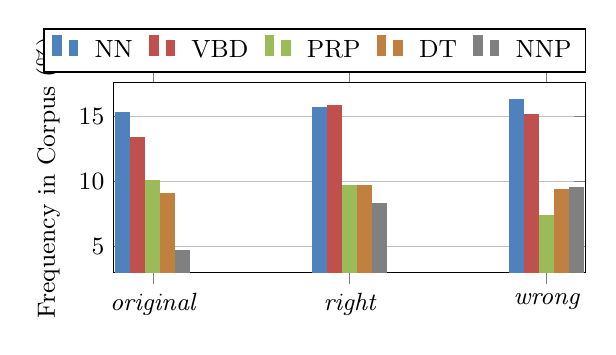
\begin{tikzpicture}
\small
    \begin{axis}[
        width  = 0.4*\textwidth,
        height = 4cm,
      %  major x tick style = transparent,
        ybar=\pgflinewidth,
        x=2.5cm,
       bar width=5pt,
        ymajorgrids = true,
        ylabel = {Frequency in Corpus (\%)},
        symbolic x coords={{\it original}, {\it right}, {\it wrong}},
        xtick = data,
        scaled y ticks = false,
        %enlarge x limits=0.25,
        ymin=3,
        legend cell align=left,
        legend style={
        		legend columns=-1,
                at={(1,1.05)},
                anchor=south east,
                column sep=1ex
        }
    ]
        \addplot[style={bblue,fill=bblue,mark=none}]
            coordinates {({\it original}, 15.3) ({\it right}, 15.7) ({\it wrong}, 16.3)};

        \addplot[style={rred,fill=rred,mark=none}]
            coordinates {({\it original}, 13.4) ({\it right}, 15.8) ({\it wrong}, 15.1)};

        \addplot[style={ggreen,fill=ggreen,mark=none}]
            coordinates {({\it original}, 10.1) ({\it right}, 9.7) ({\it wrong}, 7.4)};

        \addplot[style={brown,fill=brown,mark=none}]
            coordinates {({\it original}, 9.1) ({\it right}, 9.7) ({\it wrong}, 9.4)};

        \addplot[style={gray,fill=gray,mark=none}]
            coordinates {({\it original}, 4.7) ({\it right}, 8.3) ({\it wrong}, 9.5)};

        \legend{NN, VBD, PRP, DT, NNP}
    \end{axis}
\end{tikzpicture}
\caption{\label{roc_pos_distribution}POS tags}
\end{subfigure}
\begin{subfigure}{.5\textwidth}\center
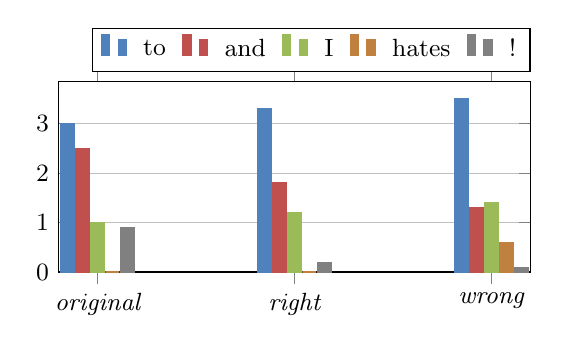
\begin{tikzpicture}
\small
    \begin{axis}[
        width  = 0.4*\textwidth,
        height = 4cm,
      %  major x tick style = transparent,
        ybar=\pgflinewidth,
        x=2.5cm,
       bar width=5pt,
        ymajorgrids = true,
%        ylabel = {Frequency in Corpus (\%)},
        symbolic x coords={{\it original}, {\it right}, {\it wrong}},
        xtick = data,
        scaled y ticks = false,
        %enlarge x limits=0.25,
        ymin=0,
        legend cell align=left,
        legend style={
        		legend columns=-1,
                at={(1,1.05)},
                anchor=south east,
                column sep=1ex
        }
    ]
        \addplot[style={bblue,fill=bblue,mark=none}]
            coordinates {({\it original}, 3) ({\it right}, 3.3) ({\it wrong}, 3.5)};

        \addplot[style={rred,fill=rred,mark=none}]
            coordinates {({\it original}, 2.5) ({\it right}, 1.8) ({\it wrong}, 1.3)};

        \addplot[style={ggreen,fill=ggreen,mark=none}]
            coordinates {({\it original}, 1) ({\it right}, 1.2) ({\it wrong}, 1.4)};

        \addplot[style={brown,fill=brown,mark=none}]
            coordinates {({\it original}, 0) ({\it right}, 0) ({\it wrong}, 0.6)};

        \addplot[style={gray,fill=gray,mark=none}]
            coordinates {({\it original}, 0.9) ({\it right}, 0.2) ({\it wrong}, 0.1)};

        \legend{to, and, I, hates, !}
    \end{axis}
\end{tikzpicture}
\caption{\label{roc_word_distribution}Words}
\end{subfigure}
\caption{The distribution of five frequent POS tags
  (\ref{roc_pos_distribution}) and words (\ref{roc_word_distribution})
  across \emph{original} endings (story cloze training set), and
  \emph{right} and \emph{wrong} endings (from the story cloze task).}

\end{figure*}


%\roy{Other things to talk about (not necessarily in that order): 
%1. no training corpus for the task. That is, the training set (a) does not contain negative example (just positive), and (b) was not generated in the same way as the positive test samples. Here you need to explicitly say that we show that we show that the training and test sets use very different styles.
%2. Maybe talk about the shared task, as well as their RepEval paper, which suggested this task as a vector-space evaluation measure?
%3. Say that the authors did an extensive work in order to  assure that the positive and negative samples are not easily distinguishable: for each pair, both endings were written by the same author (you addressed this earlier, but this seems like a better location), they tried an extensive set of baselines, showing all don't surpass a random baseline by much. Maybe now you can briefly mention the benchmarks, saying that several baselines were presented in the papers. All benchmarks attempted to learn the connection between the previous paragraph and the ending, and all performed near chance level.. However, no baseline looked at the endings independently. 
%Then you can add the benchmark text below, and conclude that this indicates that this task is well designed and hard and the one hand, but might also point to potential disagreements between the train and the test data, which we highlight in this paper.}


\isectionb{Model}

The goal of this paper is to determine the extent to which 
%does constraining authors in their writing assignments lead to them adopting different writing styles. 
different writing constraints lead the authors to adopt different writing styles. 
In order to answer these questions, we use simple methods that have been shown to be very effective for recognizing style (see \secref{Related}).
We describe our model below.

We train a logistic regression classifier to distinguish between different endings. 
Each feature vector is computed using the words in one ending, without considering earlier parts of the story. 
We use the following style features.

\begin{itemize}
\item\textit{\textbf{Length}.} The number of words in the sentence.
\item\textit{\textbf{Word n-grams.}} We use sequences of 1-5
  words. Following \citet{Tsur:2010} and \citet{Schwartz:2013}, we distinguish between high frequency and low frequency words. 
Specifically, we replace content words (nouns, verbs, adjectives, and adverbs), which are often low frequency, with their part-of-speech tags.
\item\textit{\textbf{Character $n$-grams.}} Character $n$-grams are one of the most useful features in identifying author style \cite{Stamatatos:2009}. 
We use character 4-grams.
\end{itemize}

\isectionb{Experiments}
We design two experiments to answer our research questions. 
The first is an attempt to distinguish between {\it right} and {\it wrong} endings,
the second  between {\it original} endings and new ({\it right}) endings.
We describe both experiments below.

\paragraph{Experiment 1: right/wrong endings.}
The goal of this experiment is to measure the extent to which  style features capture differences between the {\it right} and {\it wrong} endings.
As the story cloze task doesn't have a training corpus for the {\it
  right} and {\it wrong} endings (see \secref{ROC_Story}), we use the
development set as our training set, holding out 10\% for development
(3,366 training endings, 374 for development). 
 We keep the story cloze test set as is (3,742 endings).

It is worth noting that our classification task is slightly different from the story cloze task. 
Instead of classifying pairs of endings, one which is {\it right} and
another which is {\it wrong}, our classifier decides about each ending
individually, whether it is \emph{right} (positive instance) or
\emph{wrong} (negative instance).
By ignoring the coupling between {\it right} and {\it wrong} pairs, 
we are able to decrease the impact of author-specific style differences,
and focus on the difference between the styles accompanied with {\it right} and {\it wrong} writings.
\resolved{we
are able make a more general claim about the style used when writing
each of the tasks \nascomment{I'm not sure I follow this sentence; can
we be more clear?}.}

\paragraph{Experiment 2: original/new endings.}

Here the goal is to measure whether writing the ending as part of a
story imposes different style compared to writing a new ({\it right}) ending to an existing story.
We use the endings of the ROC stories as our {\it original} samples and {\it right} endings from the story cloze task   \resolved{\nascomment{if you're using the test examples as
  training data, what are you using for test? and development?  I would have thought
  you'd follow the same pattern as above ... }}as {\it new} samples.
As there are far more {\it original} instances than {\it new}
instances, we randomly select the same number of \emph{original}
instances  \resolved{\nascomment{(give the number in parentheses, for train/dev/test)} }as we have
\emph{new} instances (3,366 training endings, 374 development endings, and 3,742 test endings).
We randomly sample 5 {\it original} sets and repeat the classification experiments.
We report the average classification result.

\paragraph{Experimental setup.}
In both experiments, we add a \textsc{start} symbol at the beginning
of each sentence.\footnote{Virtually all sentences end with a period
  or an exclamation mark, so we do not add a \textsc{stop} symbol.}
For computing our features, we keep $n$-gram (character or word) features that occur at least five times in the training set.
All feature values are normalized to $[0, 1]$.
For the POS features, we tag all endings with the Spacy POS tagger.\footnote{\url{http://spacy.io/}}
We use  Python's sklearn logistic regression implementation with $L_2$
regularization, performing grid search on the development set to
tune a single hyperparameter---the regularization parameter.   \resolved{\nascomment{any other hyperparameters?  if
  not, say this is the only one.  else explain what they are.}}


\isectionb{Results}
\tabref{results} shows our results.
In Experiment 1, our model obtains 64.5\%
classification accuracy, well above a (50\%-accurate) random baseline.
\clinic{How good is this?}
\yc{how about addressing above comment from the clinic by adding a commentary such as following: This result is surprising given that our model makes the prediction based only on the last sentence without looking at the story context, thus does not have sufficient information to judge the story coherency.}
For Experiment 2, our model is even stronger, at 68.5\%.
These results indicate that an author's style is affected in an
easily-detected way when she is prompted to write (1) a \emph{wrong} story ending vs.~a
\emph{right} one, or (2) finishing her own short story vs.~someone else's.
%These numbers indicate that these different writing tasks clearly impose different writing styles on authors. 

We further measured whether these style effects are additive, by
classifying \emph{original} vs.~\emph{wrong} endings.  The setup is
exactly as in Experiment 2, but using \emph{wrong} endings instead of
\emph{right} ones.  The result is that the effects are somewhat
additive:  this third classifier achieves 75.6\%.
% That is, whether the style differences between {\it right} endings and {\it wrong} ones are different from the differences between {\it right} and {\it original} endings.
% We repeated Experiment 2, this time comparing between {\it original} and {\it wrong} sentences. 
% Our hypothesis is that differences would be even clearer. 
% Our results (\figref{results}) show that this is indeed the case: the classifier's accuracy jumps to 75.2\%.

 \resolved{
\begin{figure}
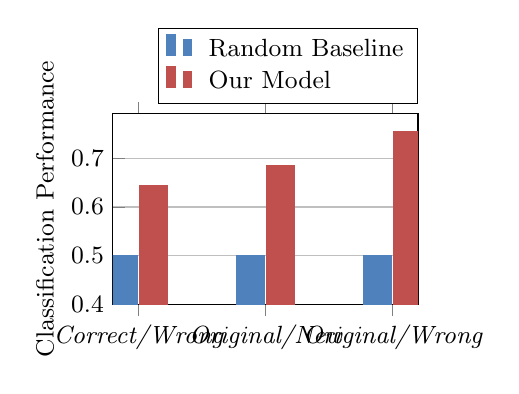
\begin{tikzpicture}
\small
    \begin{axis}[
        width  = 0.45*\textwidth,
        height = 4cm,
      %  major x tick style = transparent,
        ybar=2*\pgflinewidth,
       % bar width=14pt,
        ymajorgrids = true,
        ylabel = {Classification Performance},
        symbolic x coords={{\it Correct/Wrong}, {\it Original/New}, {\it Original/Wrong}},
        xtick = data,
        scaled y ticks = false,
        %enlarge x limits=0.25,
        ymin=0.4,
        legend cell align=left,
        legend style={
                at={(1,1.05)},
                anchor=south east,
                column sep=1ex
        }
    ]
        \addplot[style={bblue,fill=bblue,mark=none}]
            coordinates {({\it Correct/Wrong}, 0.5) ({\it Original/New}, 0.5) ({\it Original/Wrong},.5)};

        \addplot[style={rred,fill=rred,mark=none}]
            coordinates {({\it Correct/Wrong}, 0.645) ({\it Original/New}, 0.685) ({\it Original/Wrong},0.756)};

        \legend{Random Baseline, Our Model}
    \end{axis}
\end{tikzpicture}
\caption{\label{results} Results of  experiments 1 and 2 (left two charts). 
Rightmost graph shows a control experiment which classifies {\it
  original} endings vs \textit{\textbf{wrong}}
endings. \nascomment{this is overkill.  I suggest replacing it with a
  table that just shows our model, no baseline, and reiterate in the
  caption that our setup implies a 50\%-accurate random baseline.
  Also, I like including the third comparison, but I don't
  see how it's a ``control.'' }}
\end{figure}
}


\begin{table}[!t]
\begin{center}
%\small
\begin{tabular}{|c|c|} \hline
{\bf Experiment} & {\bf Accuracy} \\ \hline
{\sl right vs. wrong} & 64.5\% \\ \hline
{\sl original vs. right} & 68.5\% \\ \hline
{\sl original vs. wrong} & 75.6\% \\ \hline
\end{tabular}
\end{center}
\caption{\label{results} Results of  experiments 1 ({\it right vs. wrong}) and 2 ({\it original vs. right}). 
Bottom row shows an additional experiment which classifies {\it  original} endings vs \textit{{wrong}} endings.
In all cases, our setup implies a 50\% random baseline.}
\end{table}

\paragraph{Story cloze task.}
The results of Experiment 1 indicate that {\it right} and {\it wrong} endings are characterized by different styles.
In order to further estimate the quality of our classification results, we tackle the story cloze task using our classifier.
This classification task is more constrained than Experiment 1, as two
endings are given and the question is which is \emph{right} and which is
\emph{wrong}.
We apply the classifier from Experiment 1 as follows:
if it assigns different labels to the two given endings, we keep
them.  If not, the label whose posterior probability is lower is reversed.

\tabref{cloze_results} shows our results on the story cloze test
set. Our classifier obtains 72.4\% accuracy, 12.5\% higher than the
published state-of-the-art result on the task \cite{Salle:2016}\resolved{\nascomment{cite that here}}.
Importantly, unlike previous approaches, our classifier does not require the story corpus training data, and in fact doesn't even consider the first four sentences of the story in question.
These numbers further support the claim that the styles of {\it right} and {\it wrong} endings are indeed very different.

 \resolved{\nascomment{I suppressed the sentences about the LSDSem shared task;
  once, in the earlier footnote, is enough.}}
% Other than the published works that tackled this task, a few  recent works published their results in the LSDSem shared task website.\footnote{\url{https://competitions.codalab.org/competitions/15333}} 
% At the time of submission, our results are still state-of-the-art (though by a  smaller margin). 
% No other information other than the name of the groups and their results is available.

\begin{table}[!t]
\begin{center}
%\small
\begin{tabular}{|l|r|} \hline
{\bf Model} & {\bf Accu} \\ \hline
$\dagger${DSSM} \cite{Mostafazadeh:2016} & 0.585 \\ 
$\dagger${LexVec} \cite{Salle:2016} & 0.599 \\ \hline\hline
%{Niko (shared task)}	& 0.700\\ 
%{tbmihaylov (shared task)} & 0.711\\ \hline\hline
$\dagger${RNN}		& 0.677 \\ 
{\bf Ours} & {\bf 0.724} \\ 
$\dagger${\bf Combined (ours + RNN)} & {\bf 0.752} \\ \hline\hline
$\dagger$Human judgment & 1.000 \\ \hline
\end{tabular}
\end{center}
\caption{\label{cloze_results}
\yc{we should change accuracy to be in 0-100\% scale to be consistent with Table 2}
Results on the test set of the  story cloze task. 
The first block are published results, 
the second block is our results.
LexVec results are taken from \cite{Speer:2016}.
%RNN is our implementation. 
Human judgement scores are taken from \cite{Mostafazadeh:2016}.
Methods marked with ($\dagger$) use the story context in order to make a prediction. 
 \resolved{\nascomment{I added 0s to ``Niko'' result
  and ``human''
  so sig. digits would line up.  if we don't have sig digits for some
  of them, make the zeros white so the numbers line up.  where did the
human judgments come from?  those are not mentioned in our text anywhere!}
}}
\end{table}


\paragraph{Combination with a neural language model.}
We investigate whether our model can benefit from state-of-the-art text comprehension models, for which this task was designed. 
Specifically, we experiment with an LSTM-based \cite{hochreiter1997long} recurrent neural network language model (RNNLM; \citealp{mikolov2010recurrent}). % on the ROC story corpus training data,
%and use it to compute the probability of both {\it right} and {\it wrong} endings in the story cloze test set.
Unlike the model in this paper, which only considers the story endings, this language model follows the protocol suggested by the story cloze task designers, and harnesses their ROC Stories training set, which consists of single-ending stories, 
as well as the story context for each pair of endings. 
We show that adding our features to this powerful language model
gives improvements over our classifier as well as the language
model.  \resolved{\nascomment{reworded.  more important that our features help
  the language model, than the other way around!}}


We train the RNNLM using a single-layer LSTM of hidden dimension 512.
We use the ROC stories for training,\footnote{We use the extended, 100K stories corpus (see \secref{ROC_Story}).} setting aside 10\% for validation of the language model. 
We replace all words occurring less than 3 times with a special
out-of-vocabulary character, yielding a vocabulary size of  21,582.
Only during training, we apply a dropout rate of 60\% while running the LSTM over all 5 sentences of the stories. 
Using the Adam optimizer \cite{kingma2014adam} and a learning rate of
$\eta=.001$, we train to minimize cross-entropy. % minibatches of $50$ stories.
% h=512, dropout rate of 60%, V=21582, 10% validation set

To apply the language model to the classification problem, we select
as \emph{right} the ending with the higher value of
\begin{equation}
\frac{p_\theta(\textrm{ending} \mid
  \textrm{story})}{p_\theta(\textrm{ending})} \label{eq:ratio}
\end{equation}
The intuition is that a \emph{right} ending should be unsurprising (to
the model)
given the four preceding sentences of the story (the numerator), controlling for the
inherent surprisingness of the words in that ending (the denominator).

\nascomment{please check the paragraph above.  we need to say how we
  use the LM before we evaluate it!  also, has anyone tried an approach like this
  before?  even if we aren't exactly replicating another paper, if
  someone else used RNNs for this task, we should credit them.}
  \roy{Ours is the first work to publish LSTM results on this dataset.}

% Eval
On its own, our neural language model performs moderately well on the story cloze test. 
%This is not surprising, as \citet{Mostafazadeh:2016} hinted  that
%simple language models are insufficient.
Selecting endings based on $p_\theta(\textrm{ending} \mid \textrm{story})$ (i.e., the numerator of
Equation~\ref{eq:ratio}), we obtained only 55\% accuracy.   The ratio
in Equation~\ref{eq:ratio} achieves 67.7\%  (see
\tabref{cloze_results}).\footnote{Further analysis of this large
  difference is out of the scope of this paper, but suggests careful
  study of suitable probabilistic inference methods for such tasks.}

We combine our linear model with the RNNLM by adding three features to
our classifier: the numerator, denominator, and ratio in
Equation~\ref{eq:ratio}. % $p_\theta(ending|story),p_\theta(ending)$ and $\frac{p_\theta(ending|story)}{p_\theta(ending)}$.
We retrain our linear  model with the new feature set, and gain 2.8\%
absolute, reaching 75.2\% (15.3\% better than the published state-of-the-art\com{ and 4.1\% better than the best unpublished} result).\roy{As now the codalab shared task table contains our numbers, I removed the references to these works, and left only the footnote earlier which says that there are higher, unpublished numbers.}
These results indicate that context-ignorant style features can be used to obtain high
accuracy on the task, adding value even when context and a large
training dataset are used.  \resolved{\nascomment{check reframing here}}




\isection{Further Analysis}{Ablation}

 \resolved{\nascomment{these aren't just ablations, so I retitled}}

\subsection{Most Discriminative Feature Types}
A natural question that follows this study is which style features are most
helpful in detecting the underlying task an author was asked
to perform. 
To answer this question, we re-ran Experiment 1 with different sub-groups of features. 
\tabref{subgroups} shows our results. Results show that  character $n$-grams are the most effective style predictors, reaching within  0.6\% of the full model, but that word $n$-grams also capture much of the signal, yielding 61.2\%, which is only 3.3\% worse than the full model. 
These findings are in line with previous work that used character $n$-grams along with other types of features to predict writing  style \cite{Schwartz:2013}.


\begin{table}[!t]
\begin{center}
%\small
\begin{tabular}{|c|c|} \hline
{\bf Feature Type} & {\bf Accuracy}\\ \hline
Word $n$-grams & 0.612 \\ \hline
Character $n$-grams & 0.639 \\ \hline
Full model & 0.645 \\ \hline

\end{tabular}
\end{center}
\caption{\label{subgroups}
Results on Experiment 1 with different subsets of features.
}
\end{table}

\subsection{Most Salient Features}
A followup question is which individual features contribute most to the classification process,
as these could shed light on the stylistic differences imposed by each of the writing tasks.

In order to answer this question, we consider the highest absolute positive and negative coefficients in the logistic regression classifier in both Experiments 1 and 2, an  approach widely used  as a method of extracting the most salient features \cite{Nguyen:2013,Burke:2013,Brooks:2013}.\footnote{Although it is worth noting that its reliability is not entirely clear \cite{Yano:2012}.}
We consider only features appearing in at least 5\% of the endings in our training set. 

\paragraph{Experiment 1.}
\tabref{exp1_features} shows the most salient features for {\it right} (coherent) and {\it wrong} (incoherent) endings in Experiment 1,
along with their corpus frequency. 
The table shows a few interesting trends. 
First, authors tend to structure their sentences differently when writing {coherent}  vs.~{incoherent} endings.
For instance, {incoherent} endings are more likely to start with a proper noun and end with a common noun, 
while coherent endings have a greater tendency to end with a past tense verb.

Second, {\it right} endings will make wider use of coordination structures, as well as adjectives.
The latter might indicate that writing coherent stories imposes the authors to write more descriptive text compared to incoherent ones, 
as is the case in truthful vs.~deceptive text \cite{ott2011finding}.
Finally, we notice a few syntactic differences: {\it right} endings will more often use infinite verb structure, while {\it wrong} endings will prefer gerunds (VBG). 
\nascomment{note to self to come back
  to this after we agree on methodology.}


\com{More interestingly, the different writing tasks seem to impose a specific sentiment on the writer. 
Three of the top four most salient features for detecting {\it wrong} endings are variants of the verb ``hate''.
This indicates that when authors are asked to write {\it wrong} text, they tend to use negative language.

An alternative explanation to this hypothesis might be that the first four sentences of the stories in the ROC story corpus tend to be positive, and thus in order to make an ending {\it wrong}, authors adopted a negative approach. 
A similar idea was suggested in the original story cloze paper, where two sentiment-based baselines were evaluated. 
These baselines measured the relative sentiment between the ending and the previous sentences.
The performance of both these baselines was roughly chance-level, which seems to suggest that this is not entirely the case.
\resolved{\yc{Is it really because there's no statistical tendency in the original stories to have happy endings, as opposed to the alternative possibility --- the sentiment classifier used by Monstafazadeh 2016 didn't quite nail down the optimal feature encodings?}} \roy{this is definitely an option, and that's partly why I used hedging (``seems to suggest''). Tones it down a bit more.}}

\begin{table}[!t]
\begin{center}
%\small
\begin{tabular}{|c|c||c|c|} \hline
\textit{\textbf{Right}} & Freq. & \textit{\textbf{Wrong}}& Freq. \\ \hline
`ed .' & {\color{white}{0}}6.5\%& START NNP & 54.8\%\\ \hline
`and ' & 13.6\%& NN . & 47.5\% \\ \hline
JJ & 45.8\% & NN NN . & {\color{white}{0}}5.1\%\\ \hline
to VB & 20.1\%& VBG & 10.1\%\\ \hline
`d th' & 10.9\%& START NNP VBD & 41.9\%\\ \hline
%`ally' & 3.3\% & `hate' & {\color{white}{0}}1.9\% \\ \hline
%VBD the NN .& 2.2\% & ` hat' & {\color{white}{0}}2.0\% \\ \hline
%START RB & 3.1\% & START NNP & 54.8\% \\ \hline
%`ved ' &4.1\%&  `ated' & {\color{white}{0}}3.0\%\\ \hline
%` tim' &2.6\%&  NN . & 47.5\%\\ \hline

\end{tabular}
\end{center}
\caption{\label{exp1_features}
The top 5 most discriminative features for predicting {\it right} vs.~{\it wrong} endings,
along with their frequency in our story cloze training set.
}
\end{table}



\paragraph{Experiment 2.}
%In order to understand which features were most salient, we repeated Experiment 1, this time running SVM with L1 norm, such that it generates a sparse separating hyperplane. 
%This came at a minor cost of less than 2\% in performance compared to our L2 results (0.697 compared to 0.724).  
\tabref{exp2_features} shows the same analysis for Experiment 2.
As noted in \secref{ROC_Story}, {\it original} endings tend to be much longer, which is indeed the most salient feature for them.
This is inline with similar findings in the deception detection literature \cite{qin2004exploratory}.
An interesting observation is that exclamation marks are a strong indication for  {\it original} ending. 
This indicates that authors are more likely to show enthusiasm when writing their own text compared to ending an existing task.

Finally, when comparing the two groups of salient features from both experiments, we find an interesting trend.
Several features, such as ``START NNP'' and  ``NN .'', which indicate {\it wrong} sentences in Experiment 1, are used to predict {\it new} (i.e., {\it correct}) endings in Experiment 2. 
This indicates that, for instance, incoherent endings have a stronger tendency to begin with a proper noun compared to coherent endings, 
which in turn are more likely to do so than original endings. 
This partially explains why distinguishing between {\it original} and {\it wrong} endings is an easier task compared to the other pairs (\secref{Results}).


\setlength\tabcolsep{.15cm}
\begin{table}[!t]
\begin{center}
%\small
\begin{tabular}{|p{1.25cm}|c||p{2.9cm}|c|} \hline
\textit{\textbf{Original}} & Freq. & \textit{\textbf{New}}& Freq. \\ \hline
{\it length} & {\color{white}{.}}100.0\% & `.' & 93.0\%\\ \hline
`!' & {\color{white}{00}}6.1\%& START NNP  & 39.2\% \\ \hline
NN & {\color{white}{00}}78.9\% & START NNP VBD &29.0\% \\ \hline
RB & {\color{white}{0}}44.7\%& NN . & 42.3\% \\ \hline
`,' & {\color{white}{0}}12.7\%&  the NN . & 10.6\% \\ \hline

\end{tabular}
\end{center}
\caption{\label{exp2_features}
The top 5 most discriminative features for predicting {\it original} vs.~{\it new} ({\it right}) endings.
}
\end{table}


\isectionb{Discussion}

\paragraph{The effect of writing tasks on mental states.}
In this paper we have shown that giving a writer different writing tasks affects writing style in easily detected ways.
Our results indicate that when authors are asked to write the last
sentence of a five sentence story, they will use different style to
write a {\it right} ending compared to a {\it wrong} ending. We have
also shown that writing the ending as part of one's own five-sentence story is very different than reading four sentences and then writing the fifth.
Our findings hint that the nature of the writing task imposes a
different mental state on the author, which is expressed in ways which
are often implicit, but can be observed using extremely simple automatic tools. 

Previous work have shown that  writing task could affect mental states.
For instance, several works demonstrated that writing deceptive text leads to a significant cognitive burden \cite{Newman:2003,Banerjee:2014}.
These works have also shown that this burden is accompanied by different writing style compared to truthful text.
Other studies have shown that writing tasks can even have a long term effect,
by showing that writing emotional texts can benefit both physical and mental health \cite{Lepore:2002,Frattaroli:2006}. 
\citet{Campbell:2003} also showed that the health benefits of writing emotional text are accompanied by changes in writing style, mostly in the use of pronouns.

Another line of works has shown that writing style is affected by the mental state.
First, the author's personality traits (e.g., depression, neuroticism, narcissism) affect her writing style \cite{schwartz2013personality,Ireland:2014b}.
Second, temporary changes, such as a romantic relationship \cite{Ireland:2011,Bowen:2016}, work collaboration \cite{Tausczik:2009,Gonzales:2009} or negotiation \cite{Ireland:2014} may also affect writing style.
Finally, writing style can also change from one sentence to another, for instance between positive and negative text \cite{Davidov:2010} or when writing sarcastic text \cite{Tsur:2010}. 

This large body of works indicates a tight connection between writing tasks, mental states and different writing styles.
This connection hints that the link discovered in this paper, between the different writing tasks and the resulting difference in writing style, also goes through a change in mental state. 
Nonetheless, further investigation is required in order to further validate this hypothesis.


\paragraph{The story cloze task.}
This paper also provides important insights for the future design of NLP tasks. 
The story cloze task was very carefully designed. Many factors, such as the topic diversity, as well as  temporal and causal relation diversity,  were controlled for \cite{Mostafazadeh:2016}. 
The authors also made sure each pair of endings was written by the same author, partly in order to avoid author specific style effects.
 Nonetheless, this paper shows that despite these efforts, several significant style differences are found between the training and the test set, as well as between the positive and negative labels. 
 
The findings in this paper suggest that careful attention must be paid to instructions given to authors, especially in unnatural tasks such as writing a {\it wrong} ending. 
One way to avoid such problems is by using shorter text spans, such as the ones used in the Winograd schema \cite{Levesque:2011}.
A different approach is to use naturally occurring text, as used in recent machine reading tasks (see \secref{Related}). 
%However,  these approaches have their shortcomings, and do not capture the same signal as intended by the author of the story cloze task.
A way to avoid the inherent biases people have when writing is to rather than ask them to write text, have them rate sentences for naturally occurring text by parameters such as coherence (or very differently -- the level of surprise).

\com{
Another lesson from this paper relates to baseline methods. 
The authors of the story cloze task experimented with a wide and diverse set of baselines, including n-gram baselines, word embeddings baselines, sentiment baselines, and narrative chain baselines. 
Nonetheless, running preliminary tests on the data, such as average length or  POS and word distribution,  could have revealed potentially unwanted phenomena in the data.
\resolved{\nascomment{this paragraph needs extra care.  the authors of the ROC
  paper did try to control for a lot of things and they did run
  baselines.  we ought to be generous and reiterate that here.  what,
  precisely, did they miss?  the lesson isn't just ``run more controls
  and baselines'' is it?}
First, it stresses the need to carefully control for even seemingly minor details. 
Second, it emphasizes the importance of running baseline models.
While recent advances in NLP  suggest that many classic NLP methods are out-of-date, 
this is not necessarily the case, especially for small
datasets. \nascomment{ this bit about simple models feels like a red herring}}
This is particularly important in order to ensure that  new technological improvements are capturing a qualitatively different signal.
The substantial improvement we get when combining our model
with the RNN language model (\secref{Experiments}) suggests that
despite the high results obtained by the simple model, 
methods that exploit the wider context  capture a different aspect of the
task. \resolved{\nascomment{I like ending on this happier note, but let's not
  call it ``luck'' and let's focus on the task and representations,
  not the ML methods, which are probably not the heart of the difference}}
  \roy{Modified this to be more concrete. Did end up hinting that they should have done a better job at analyzing their data before publishing. Feel free to tone down.}
}
\roy{Commented out the lessons about the importance of running baselines.}
\isection{Related Work}{Related}

\paragraph{Writing style.}
Writing style has been an active topic of research for decades. 
The models used to characterize style are often linear classifiers with style features such as character and word $n$-grams \cite{Stamatatos:2009,Koppel:2009}.
Previous work has shown that different authors can be grouped by their
writing style, according to factors such as age
\cite{Pennebaker:2003,Argamon:2003,Schler:2006,Rosenthal:2011,nguyen:2011:latech},
gender \cite{Argamon:2003,Schler:2006,bamman2014gender}, and native language
\cite{Koppel:2005,Tsur:2007,Bergsma:2012}.   \resolved{\nascomment{cite generously here, it costs us nothing}}
At the extreme case, each individual author adopts a unique writing
style \cite{mosteller1963inference,pennebaker1999linguistic,Schwartz:2013}. 
\com{Interestingly, previous work has shown that individual style can be affected from coarse-grained factors such as those just described, but also from other less apparent factors such as mental state, or even living in a high-elevation location \cite{schwartz2013personality}.

Unlike the works just described which compare the writing style
between different authors, some works have shown that the same author
can adopt a different style used when writing positive vs.~negative
text \cite{Davidov:2010} or when writing sarcastic text \cite{Tsur:2010}. In this work, we have shown that the same author can adopt a different style when facing different writing tasks.}

The line of work that most resembles our work is the detection of deceptive text. 
Several researchers have used stylometric features to  predict deception 
\cite{Newman:2003,hancock2007lying,ott2011finding,Feng:2012}.
Some works even showed that writing style applied when lying is different across genders \cite{Perez:2014a,Perez:2014b}.
In this work, we have shown that an even more subtle writing task---writing {coherent} and {incoherent} story endings---imposes different styles on the author.


\paragraph{Machine reading.}
The  story cloze task, which is the focus of this paper, is part of a wide set of machine reading works published in the last few years.
These include datasets like bAbI \cite{Weston:2015}, SNLI \cite{bowman2015large}, CNN/DailyMail \cite{hermann2015teaching}, SQuAD \cite{rajpurkar2016squad}, and LAMBADA \cite{Paperno:2016}. 

While these works have presented valuable resources for researchers, 
it is often the case that these datasets suffer from methodological
problems caused by applying noisy automatic tools to generate them\nascomment{this is not clear to me, what does it mean?} \roy{better?}\cite{Chen:2016}. 
In this paper we have pointed to another methodological challenge in
designing machine reading tasks, namely that different writing tasks
used to generated the data affect the writing style of the positive
and negative samples, confounding the classification problem.
%, as well as create a discrepancy between the training and the test data.
 \resolved{\nascomment{dropped the train/test discrepancy here}}

\isectionb{Conclusion}

The research question that guided this work is the extent to which different writing tasks result in different writing styles.
We experimented with the story cloze task, which introduces two interesting comparison points: %setups for our purposes:
%a setup where the same author writes both a {\it right} and an {\it wrong} ending to a story, 
%and one which compares an ending written as part of a story to a standalone ending added to a story written by someone else.
 the difference between writing a story on one's own and continuing someone else's story,
 and the difference between writing a coherent and an incoherent story ending.
In both cases, a simple linear model reveals measurable differences in writing styles, %that different styles are imposed.
%The different styles allow our style detection 
which in turn allows our final 
model to achieve state-of-the-art results on the story cloze task.

The findings presented in this paper have  cognitive implications, as
they motivate further research on the exact effect that a writing
prompt has on an author's mental state, and also her concrete response.
They also provide valuable lessons for designing new NLP datasets.
 \resolved{\nascomment{drop the last sentence, it makes this paper seem less
  complete} Future work will include testing whether other similar writing tasks, such as fake news, also impose their own unique and identifiable style on their authors.}




% include your own bib file like this:
%\bibliographystyle{acl}
%\bibliography{acl2017}

\bibliography{acl2017}
\bibliographystyle{acl_natbib}

\end{document}
